\documentclass{article}

\usepackage{geometry}
\usepackage{flafter}
\usepackage{listings}
\usepackage{graphicx}
\usepackage{tcolorbox}
\usepackage{textcomp}
\usepackage{gensymb}
\usepackage{indentfirst}
\usepackage{romannum}
\usepackage{vhistory}
\usepackage{cprotect}
\usepackage{hyperref}

% change margins
\geometry{letterpaper, portrait, margin=1in}

% graphics in images/ folder
\graphicspath{ {images/} }
 
% for lstlisting code environment
\lstdefinestyle{bashstyle}{
  language=bash,
  basicstyle=\ttfamily,
  keywordstyle=\color{blue},
  commentstyle=\color{green},
  numberstyle=\tiny\color{gray},
  numbers=left,
  breaklines=true
}

% settings for /href
\hypersetup{
    colorlinks=true,
    linkcolor=black,
    filecolor=magenta,
    urlcolor=blue,
}

\title{RoboJackets Training Firmware Setup Guide}
\author{Andrew Roach}
\date{\today\\v1.1}

%%%%%%%%%%%%%%%%%%%%%%%%%%%%%%%%%%%%%%%%%%%%%%%%%%%%%%%%%%%%%%%%%%%%%%%%%%%%%%%%%%%%%%%%%%%%%%%%%%
%% NOTE TO EDITOR:                                                                              %%
%% 1. Please update the version number and the version history when making changes.             %%
%% 2. This is a living document. If the hardware or software requirements change, this document %%
%%      should change.                                                                          %%
%% 3. Keep it simple! Don't include unnecessary or extraneous information. Try to minimize      %%
%%      linking to external websites; explain everything the reader needs to know clearly and   %%
%%      concisely.                                                                              %%
%%%%%%%%%%%%%%%%%%%%%%%%%%%%%%%%%%%%%%%%%%%%%%%%%%%%%%%%%%%%%%%%%%%%%%%%%%%%%%%%%%%%%%%%%%%%%%%%%%

\begin{document}
\maketitle{}
\setcounter{tocdepth}{2}
\tableofcontents
\pagebreak

\begin{versionhistory}
  \vhEntry{1.0}{9/22/23}{Andrew Roach}{Created}
  \vhEntry{1.1}{10/6/23}{Andrew Roach}{Removed section on Verifying CH340 drivers, added section on updating Arduino Nano bootloader.}
\end{versionhistory}

\clearpage

\section{Installing the Arduino IDE}

We will be using the legacy version of the Arduino IDE (version 1.8.19). Follow the installation instructions based on your platform.

\subsection{Windows and Mac}

\begin{enumerate}
    \item Go to \url{https://www.arduino.cc/en/software} and scroll down to ``Legacy IDE (1.8.X)''. Download the binary corresponding to your platform.
    \item Run the installer. Allow the installer to install everything, including drivers.
\end{enumerate}

\subsection{Linux}

\begin{enumerate}
    \item Go to \url{https://www.arduino.cc/en/software} and scroll down to the ``Legacy IDE (1.8.X)''. The Linux Arduino IDE should download as a \verb|tar.xz| file.
    \item Run the following commands, replacing \verb|<arduino-ide>| with the name of the downloaded file.
    \begin{lstlisting}[style=bashstyle, label=lst:mybashcode]
    tar -xJvf <arduino-ide>.tar.xz -C /home/$(whoami)
    cd /home/$(whoami)/<arduino-ide>
    sudo ./install.sh
    \end{lstlisting}
\end{enumerate}

\newpage

% \section{Verify CH340 Drivers}

% Our Arduino Nanos are kinda old, so they often don't work out of the box without installing the correct drivers first. Your operating system or the installation of the Arduino IDE might have installed the correct drivers, so it's a good idea to check if you have the driver before reinstalling them.

% \subsection{Checking CH340 Drivers on Windows}

% {\bf Checking if driver is present: } type \verb|driverquery| into the command prompt. You should see a driver called \verb|CH341SER|. 

% \begin{figure}[ht]
%     \centering
%     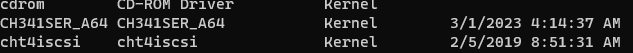
\includegraphics[width = 0.7\textwidth]{images/windows-module-present.png}
%     \cprotect\caption{Output of the command \verb|driverquery| on Windows system. \verb|CH341SER| driver module is present.}
% \end{figure}

% \vspace{1em}

% {\bf Checking if driver loads: } Plug the Arduino Nano into your computer. Go to \verb|Device Manager| and look under \verb|Ports|. You should see the Arduino Nano as \verb|USB-SERIAL CH340|, followed by the \verb|COM| port it's associated with.

% \begin{figure}[ht]
%     \centering
%     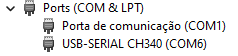
\includegraphics[width = 0.4\textwidth]{images/windows-module-load-correct.png}
%     \cprotect\caption{Windows Device Manager displaying Arduino Nano plugged into COM6}
% \end{figure}

% \begin{figure}[ht]
%     \centering
%     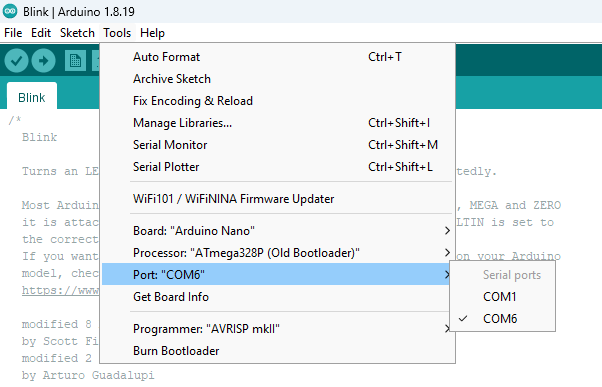
\includegraphics[width = 0.7\textwidth]{images/windows-arduino-ready.png}
%     \cprotect\caption{Arduino IDE on Windows with Arduino Nano plugged in. If the driver has been installed correctly, you should see the Arduino Nano show up in the Arduino IDE under \verb|Tools > Port| which matches the COM port in Device Manager.}
% \end{figure}

% \newpage

% \subsection{Checking CH340 Drivers on Linux}

% {\bf Checking if module is present: } type \verb|modinfo ch341| into your shell. The command should return a bunch of information about the \verb|ch341| kernel module.

% \begin{figure}[ht]
%     \centering
%     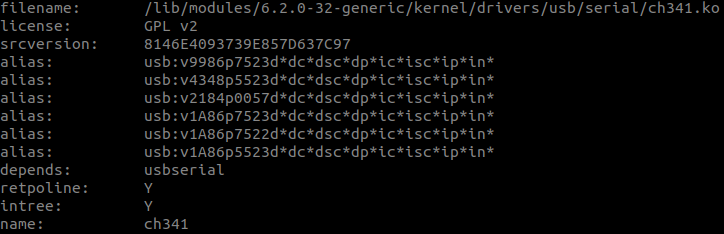
\includegraphics[width = 0.7\textwidth]{images/linux-module-present.png}
%     \cprotect\caption{Output of command \verb|modinfo ch341| on Linux system. \verb|ch341| Linux kernel module is present.}
% \end{figure}

% \vspace{1em}

% {\bf Checking if module loads: } Plug the Arduino Nano into your computer. Enter the command \verb|sudo dmesg| into your shell.

% \begin{itemize}
%     \item If you see the following, you need to uninstall \verb|brltty|. After uninstalling \verb|brltty|, unplug and plug in the Arduino Nano and run \verb|sudo dmesg| again.
%     \begin{itemize}
%         \item Ubuntu: \verb|sudo apt remove brltty|.
%     \end{itemize}

%     \begin{figure}[ht]
%         \centering
%         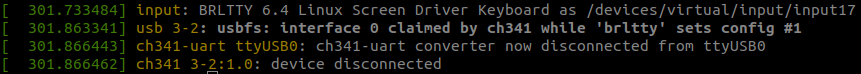
\includegraphics[width = 0.7\textwidth]{images/linux-module-load-incorrect.png}
%         \cprotect\caption{Output of command \verb|sudo dmesg| on Linux system after plugging in Arduino Nano. \verb|brltty| is interfering with the \verb|ch341| kernel module.}
%     \end{figure}
    
%     \item If you see the following, type \verb|ls /dev/tty*|. You should see the Arduino Nano show up as \verb|/dev/ttyUSB[0-9]| or \verb|/dev/ttyACM[0-9]|. This indicates that the kernel module has loaded successfully.

% \begin{figure}[ht]
%     \centering
%     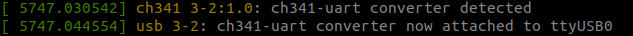
\includegraphics[width = 0.7\textwidth]{images/linux-module-load-correct.png}
%     \cprotect\caption{Output of command \verb|sudo dmesg| on Linux system after plugging in Arduino Nano. \verb|ch341| Linux kernel module has loaded correctly.}
% \end{figure}

% \begin{figure}[ht]
%     \centering
%     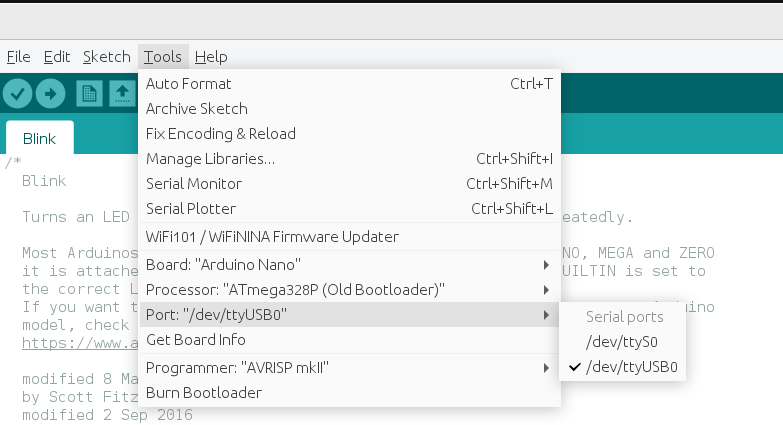
\includegraphics[width = 0.7\textwidth]{images/linux-arduino-ready.png}
%     \cprotect\caption{Arduino IDE on Linux with Arduino Nano plugged in. If the driver has been installed correctly, you should see the Arduino Nano show up in the Arduino IDE under \verb|Tools > Port| as either \verb|/dev/ttyUSB[0-9]| or \verb|/dev/ttyACM[0-9]|.}
% \end{figure}

% \end{itemize}

% \clearpage

\section{Installing CH340 Drivers}

MacOS and Linux users should have the correct drivers already, so no further action is needed. However, Windows users have to install an older driver version.

\subsection{Installing CH340 Drivers on Windows}

At the time of writing, the most recent version of the USB-SERIAL CH340/CH341 driver is v.3.8.2023.2. {\bf You must install v.3.5.2019.1!} The v.3.8.2023.2 version of the driver is incompatible with the Arduino Nanos we have! Download the driver at:
\begin{center}
    \url{https://deviceinbox.com/drivers/1571-winchiphead-usb-serial-ch340-ch341-driver.html}
\end{center}

Unzip the files and run \verb|Setup.exe|. The windows that pops up should look like {\bf Figure \ref{fig:windows-driver-setup}}. First, hit the ``Uninstall'' button to uninstall the v.3.8.2023.2 drivers, then hit the ``Install'' button to install the  v.3.5.2019.1 drivers.

\begin{figure}[ht]
    \centering
    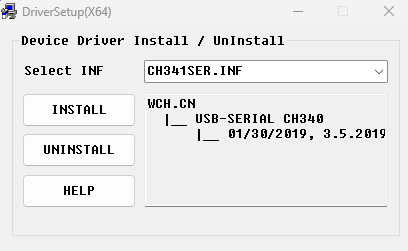
\includegraphics[width = 0.7\textwidth]{images/windows-driver-setup.png}
    \cprotect\caption{USB-SERIAL CH340/CH341 Installation on Windows 11, version 3.5.2019.1.}
    \label{fig:windows-driver-setup}
\end{figure}

% \subsection{Installing CH340 Drivers on Ubuntu Linux}

% Open a command prompt and enter the following commands:

% \begin{lstlisting}[style=bashstyle, label=lst:mybashcode, numbers = none]
% sudo apt install build-essential git
% sudo apt remove brltty
% git clone https://github.com/juliagoda/CH341SER.git CH341SER
% cd CH341SER
% make
% \end{lstlisting}

% Check if you have SecureBoot enabled by running \verb|mokutil --sb-state|. If SecureBoot is enabled, run the command: 

% \begin{lstlisting}[style=bashstyle, label=lst:mybashcode, numbers = none]
% kmodsign sha512 /var/lib/shim-signed/mok/MOK.priv /var/lib/shim-signed/mok/MOK.der ./ch34x.ko
% \end{lstlisting}

% Finally, run:

% \begin{lstlisting}[style=bashstyle, label=lst:mybashcode, numbers = none]
% make load
% \end{lstlisting}

% After installing the drivers, go to section 2.2 to verify the drivers are present.

\newpage

\section{Updating the Arduino Nano's  Bootloader}

{\bf This section is only relevant for RoboJackets trainers. Update the Arduino Nano's bootloaders in advance to avoid issues during Firmware Training.} \par

\vspace{1em}

Most offbrand Arduino Nanos have old bootloaders. To maximize compatibility, you should update their bootloaders using an Arduino Uno as a programmer.

\subsection{Setting up the Arduino Uno as a Programmer}

The following setups will set up the Arduino Uno with the \verb|ArduinoISP| example program.

\begin{enumerate}
    \item Plug an Arduino Uno R3 into your computer using a USB Type B cable.
    \item Open up the \verb|ArduinoISP| example sketch under \verb|File > Examples > ArduinoISP|.
    \item Ensure the settings under \verb|Tools| are as follows:
    \begin{itemize}
        \item Board: \verb|Arduino Uno|
        \item Port: select the port the Arduino Uno is plugged into. 
        \begin{itemize}
            \item On Windows, check the “Ports” section in Device Manager.
            \item On Linux, check for devices starting with \verb|/dev/ttyACM*| or \verb|/dev/ttyUSB*|.
        \end{itemize}
        \item Programmer: \verb|AVPISP mk|\Romannum{2}
    \end{itemize}
    \item Upload the \verb|ArduinoISP| to the Arduino Uno.
\end{enumerate}

\subsection{Wiring the Arduino Nano to the Arduino Uno Programmer}

Connect the Arduino Uno to the Arduino Nano as shown in {\bf Figure \ref{fig:wiring-diagram}}. Note that you can also connect to the Arduino Nano's ICSP pins.

\begin{figure}[ht]
    \centering
    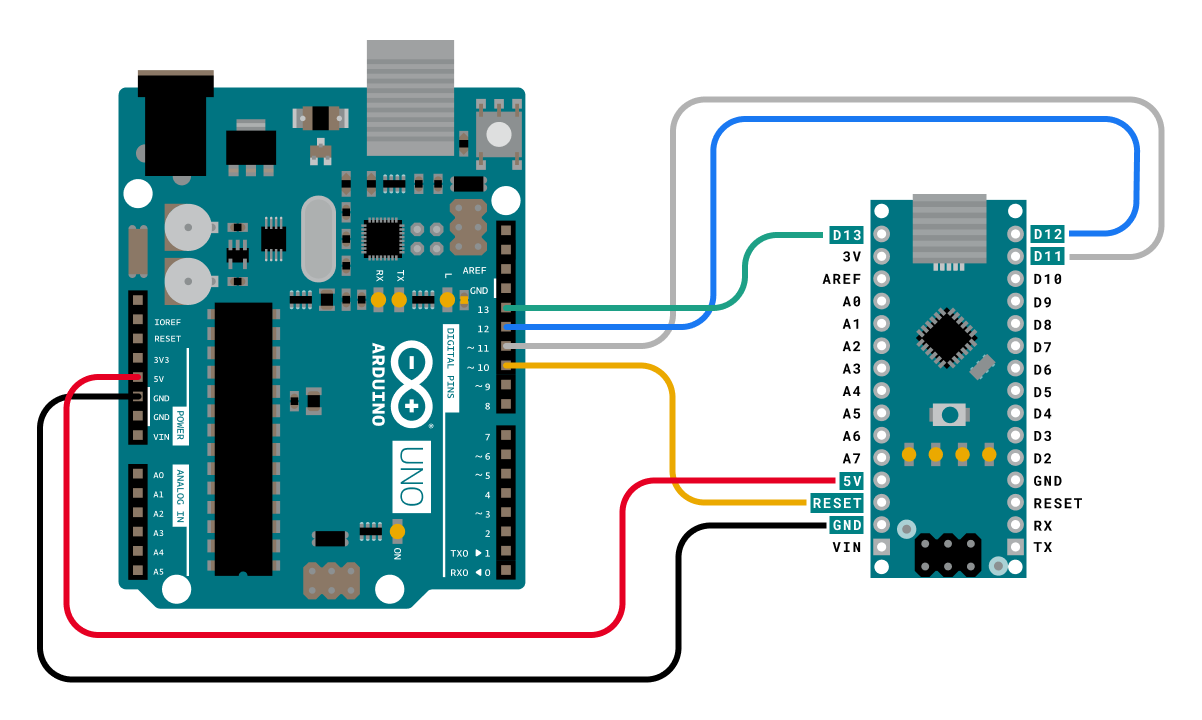
\includegraphics[width = 0.7\textwidth]{images/Uno_to_Nano_burn_bootloader.png}
    \cprotect\caption{Wiring Diagram for an Programming Arduino Nano's Bootloader using an Arduino Uno.}
    \label{fig:wiring-diagram}
\end{figure}

\clearpage

\subsection{Burning the Arduino Nano's Bootloader}

Once the Arduino Uno is wired to the Arduino Nano, follow these steps.

\begin{enumerate}
    \item {\bf Plug in the Arduino Uno into your computer}. Do NOT plug in the Arduino Nano!
    \item Ensure the settings under \verb|Tools| are as follows:
    \begin{itemize}
        \item Board: \verb|Arduino Nano|
        \item Processor: \verb|ATmega328P| 
        \begin{itemize}
            \item this setting determines which bootloader is burned onto the Arduino Nano
        \end{itemize}
        \item Port: select the port the Arduino Uno is plugged into. 
        \begin{itemize}
            \item On Windows, check the “Ports” section in Device Manager.
            \item On Linux, check for devices starting with \verb|/dev/ttyACM*| or \verb|/dev/ttyUSB*|.
        \end{itemize}
        \item Programmer: \verb|Arduino as ISP|
    \end{itemize}
    \item Under \verb|Tools|, click \verb|Burn Bootloader|. Lights on the Arduino Uno and the Arduino Nano should flash to indicate the burning process is underway. Upon completion, the Arduino IDE should say ``Done Burning bootloader''.
\end{enumerate}

Congratulations! The Arduino Nano now has the updated bootloader. You should be able to program the Arduino Nano by plugging it into the computer normally using the following settings:

\begin{itemize}
    \item Board: \verb|Arduino Nano|
    \item Processor: \verb|ATmega328P|
    \item Port: select the port the Arduino Uno is plugged into. 
    \item Programmer: \verb|AVPISP mk|\Romannum{2}
\end{itemize}
    
\end{document}